\begin{table}
    \begin{tabular}{c c c}
        \toprule
        Time (min) & Temperature (\si{\celsius}) - Cotton & Temperature (\si{\celsius}) - Aluminium \\
        \midrule
        0	&	22.6	&	22.6	\\
        1	&	23.8	&	23.3	\\
        2	&	24.5	&	24.6	\\
        3	&	25.8	&	25.5	\\
        4	&	26.7	&	26.3	\\
        5	&	27.5	&	27.1	\\
        6	&	28.5	&	27.9	\\
        7	&	29.4	&	28.9	\\
        8	&	30.1	&	29.6	\\
        9	&	30.9	&	30.6	\\
        10	&	31.9	&	30.9	\\
        11	&	33	&	31.9	\\
        12	&	--	&	32.5	\\
        13	&	--	&	33	\\        
        \bottomrule
    \end{tabular}
    \caption{Comparison between insulation methods}
\end{table}

\begin{figure}[h] %Non-insulated mixing vs non-mixing
    \begin{minipage}{0.45\textwidth}
        \centering
    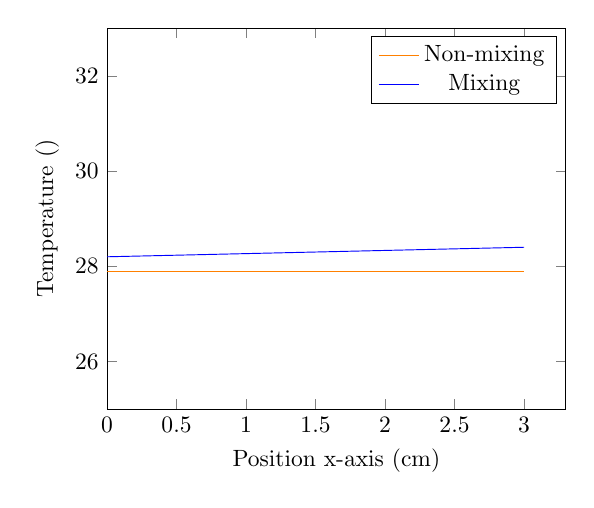
\begin{tikzpicture}[scale=0.85]
        \begin{axis}[
            xlabel= Position x-axis (cm), ylabel=Temperature (\si{\celsius}), xmin=0, ymin=25, ymax=33
        ]
        \addplot[orange] table[]{
            0.0   27.9
            1.5 27.9
            3.0 27.9
        };
        \addplot[blue] table[]{
            0.0   28.2
            1.5 28.3
            3.0 28.4
        };
        \legend{Non-mixing, Mixing}
        \end{axis}
        \end{tikzpicture}
    \end{minipage}
    \begin{minipage}{0.45\textwidth}
        \centering
        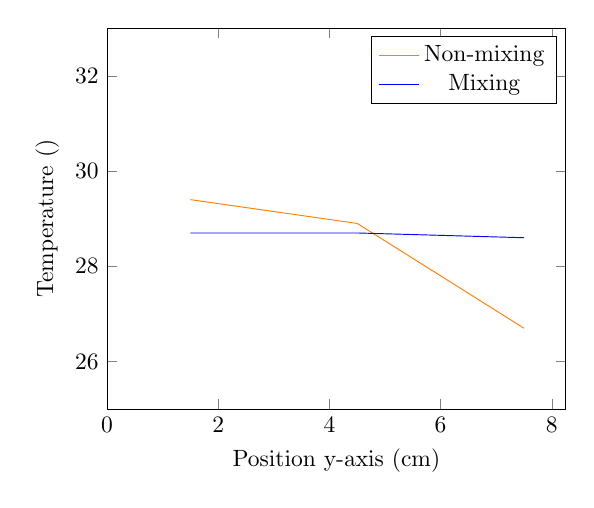
\begin{tikzpicture}[scale=0.85]
            \begin{axis}[
                xlabel= Position y-axis (cm), ylabel=Temperature (\si{\celsius}), xmin=0, ymin=25, ymax=33
            ]
                \addplot[orange] table[]{
                    1.5 29.4
                    4.5 28.9
                    7.5 26.7
                };
                \addplot[blue] table[]{
                    1.5 28.7
                    4.5 28.7
                    7.5 28.6
                };
                \legend{Non-mixing, Mixing}
            \end{axis}
        \end{tikzpicture}
    \end{minipage}
    \caption{Non-insulated, Mixing compared to Non-mixing}
	\label{fig:WithoutInsulationComparison}
\end{figure}

\begin{figure}[h] %Mixing, insulated vs non insulated
    \begin{minipage}{0.45\textwidth}
        \centering
    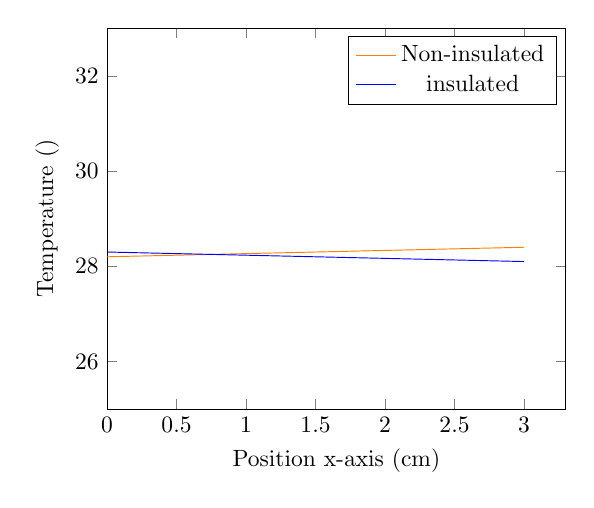
\begin{tikzpicture}[scale=0.85]
        \begin{axis}[
            xlabel= Position x-axis (cm), ylabel=Temperature (\si{\celsius}), xmin=0, ymin=25, ymax=33
        ]
        \addplot[orange] table[]{
            0   28.2
            1.5 28.3
            3.0 28.4
        };
        \addplot[blue] table[]{
            0   28.3
            1.5 28.2
            3.0 28.1
        };
        \legend{Non-insulated, insulated}
        \end{axis}
        \end{tikzpicture}
    \end{minipage}
    \begin{minipage}{0.45\textwidth}
        \centering
        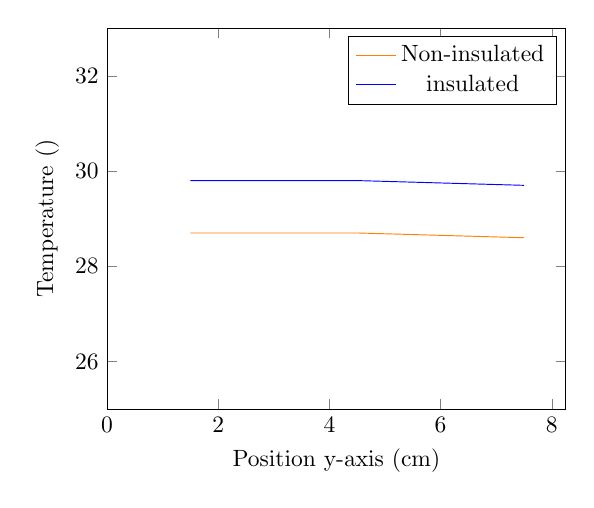
\begin{tikzpicture}[scale=0.85]
            \begin{axis}[
                xlabel= Position y-axis (cm), ylabel=Temperature (\si{\celsius}), xmin=0, ymin=25, ymax=33
            ]
                \addplot[orange] table[]{
                    1.5 28.7
                    4.5 28.7
                    7.5 28.6
                };
                \addplot[blue] table[]{
                    1.5 29.8
                    4.5 29.8
                    7.5 29.7
                };
                \legend{Non-insulated, insulated}
            \end{axis}
        \end{tikzpicture}
    \end{minipage}
    \caption{Mixing, Insulated compared to non-insulated}
	\label{fig:WithoutInsulationComparison}
\end{figure}

\begin{figure}[h] %With and without lid, 2cm insulation
    \begin{minipage}{0.45\textwidth}
        \centering
    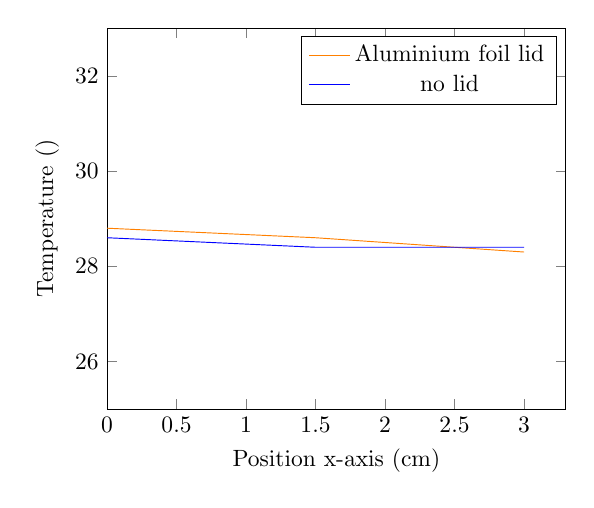
\begin{tikzpicture}[scale=0.85]
        \begin{axis}[
            xlabel= Position x-axis (cm), ylabel=Temperature (\si{\celsius}), xmin=0, ymin=25, ymax=33
        ]
        \addplot[orange] table[]{
            0   28.8
            1.5 28.6
            3.0 28.3
        };
        \addplot[blue] table[]{
            0   28.6
            1.5 28.4
            3.0 28.4
        };
        \legend{Aluminium foil lid, no lid}
        \end{axis}
        \end{tikzpicture}
    \end{minipage}
    \begin{minipage}{0.45\textwidth}
        \centering
        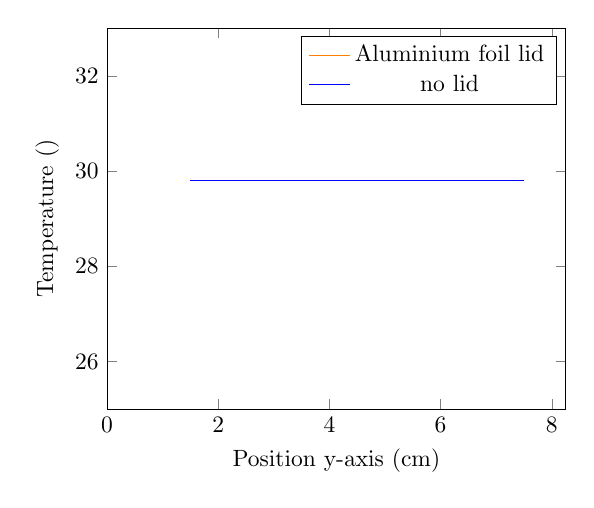
\begin{tikzpicture}[scale=0.85]
            \begin{axis}[
                xlabel= Position y-axis (cm), ylabel=Temperature (\si{\celsius}), xmin=0, ymin=25, ymax=33
            ]
                \addplot[orange] table[]{
                    1.5 29.8
                    4.5 29.8
                    7.5 29.8
                };
                \addplot[blue] table[]{
                    1.5 29.8
                    4.5 29.8
                    7.5 29.8
                };
                \legend{Aluminium foil lid, no lid}
            \end{axis}
        \end{tikzpicture}
    \end{minipage}
    \caption{2 cm thick insulation, Comparison for use of lid}
	\label{fig:WithoutInsulationComparison}
\end{figure}

\begin{figure}[h] %Optimal thickness of insulation
    \begin{minipage}{0.45\textwidth}
        \centering
    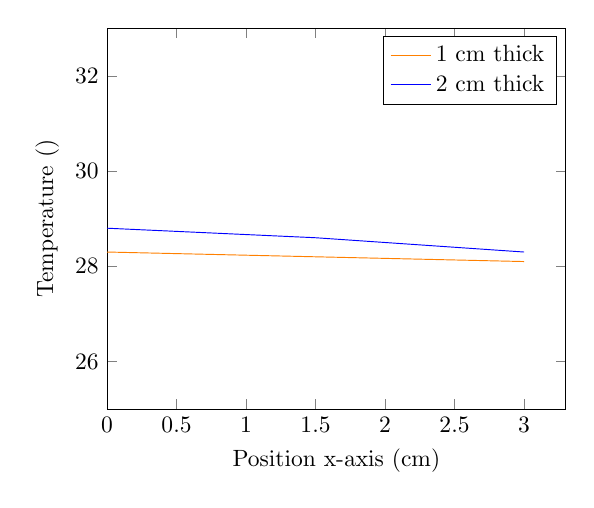
\begin{tikzpicture}[scale=0.85]
        \begin{axis}[
            xlabel= Position x-axis (cm), ylabel=Temperature (\si{\celsius}), xmin=0, ymin=25, ymax=33
        ]
        \addplot[orange] table[]{
            0   28.3
            1.5 28.2
            3.0 28.1
        };
        \addplot[blue] table[]{
            0   28.8
            1.5 28.6
            3.0 28.3
        };
        \legend{1 cm thick, 2 cm thick}
        \end{axis}
        \end{tikzpicture}
    \end{minipage}
    \begin{minipage}{0.45\textwidth}
        \centering
        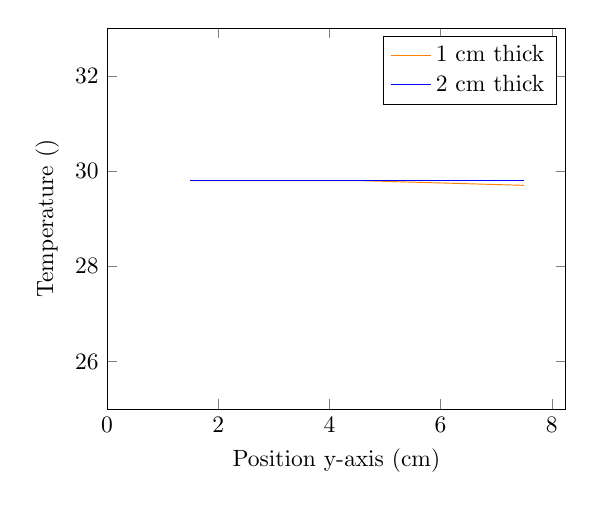
\begin{tikzpicture}[scale=0.85]
            \begin{axis}[
                xlabel= Position y-axis (cm), ylabel=Temperature (\si{\celsius}), xmin=0, ymin=25, ymax=33
            ]
                \addplot[orange] table[]{
                    1.5 29.8
                    4.5 29.8
                    7.5 29.7
                };
                \addplot[blue] table[]{
                    1.5 29.8
                    4.5 29.8
                    7.5 29.8
                };
                \legend{1 cm thick, 2 cm thick}
            \end{axis}
        \end{tikzpicture}
    \end{minipage}
    \caption{Mixing, Comparison for thickness of insulation}
	\label{fig:WithoutInsulationComparison}
\end{figure}

Comparing figures \ref{fig:NonMixing} and \ref{fig:Mixing}, although not much difference in temperature change along X-direction, the temperature change along Y-direction is significant, with a range between 26.7-29.4 \si{\celsius} and a gradient of -0.45 under non mixing condition. In comparison to that figure \ref{fig:Mixing} has a much stable gradient with a value of -0.017 under mixing condition, showing that heat is being distributed evenly along both horizontal and vertical directions within the cup. Therefore, we concluded mixing condition is required and should be included in our design in order to meet our objectives of the experiment.  

Comparing figure \ref{fig:Mixing} and \ref{fig:NonInsulated}, both graphs seems to have a steady gradient along both directions, as a result of uniform distribution of heat. The slight difference come from that graph \ref{fig:NonInsulated} is shifted upwards generally in contrast to \ref{fig:Mixing}. This suggest that a higher y-intercept and greater temperature of the system, due to less heat loss to the surroundings. Our desired temperature is around 30\si{\celsius}, as even if heat is lost or accumulated the system’s temperature is still within the range of 28-33\si{\celsius} by allowing some small fluctuations. The graph \ref{fig:NonInsulated} shows under mixing condition with insulation allows closer approach to our desired temperature, therefore we concluded that insulation is also required. Follow by that we compared \ref{fig:NonInsulated} to \ref{fig:Insulated}, where first one used 1 cm thick cotton jacket and second used 2 cm thick, the temperatures don’t have much difference vertically, however horizontally there is an increase by 0.5\si{\celsius}, which we were then able to decide 2 cm thick cotton jacket should be used. An additional experiment was conducted with an aluminium foil layer placed on the top of the bioreactor for testing, but the effect it made on minimising heat loss was insignificant.

\subsubsection{Calculations}
Temperature recorded ranged from 28 to 30 \si{\celsius}, therefore we take an average between the values for \SI{27}{\celsius} and \SI{32}{\celsius} \cite{doi:10.1063/1.555963}. Furthermore, the cup is a truncated cone, and therefore its area can be calculated as:
\begin{equation}
    \begin{split}
        A &= (5+3)\pi \sqrt{{(5-3)}^2} + 8^2 = \SI{0.0207}{\meter} \\
        k_w &= \SI{0.614}{\watt\per\meter\per\celsius}
    \end{split}
\end{equation}

Utilising Fourier's law of heat, equation (\ref{eq:HeatFlux}), we calculate heat flux in each direction and summarise in Table \ref{tb:HeatFlux}.

\begin{table}
    \begin{tabular}{c c c}
        \toprule
         & Heat flux (x-direction) $\si{\watt} \cdot 10^{-4}$ & Heat flux (y-direction) $(\si{\watt}) \cdot 10^{-4}$ \\
        \midrule
        1 cm thick cotton	&	8.48	&	2.12	\\
        Without insulation	&	-8.48	&	2.12	\\
        \bottomrule
    \end{tabular}
    \caption{Heat flux under different conditions}
    \label{tb:HeatFlux}
\end{table}

From Table \ref{tb:HeatFlux}, it can be observed that heat induction with insulation and without insulation don't seem to have much difference here, with a magnitude of $10^{-8}$. This difference may be really small, but as this prototype is a lab scale of the bioreactor, the difference in an industry size reactor can be huge therefore cannot be ignored. We can conclude that insulation is better at keeping the temperature constant, and it will make a significant difference on large scale. One consideration for scaling this prototype is that it is neither efficient nor possible to reactor with 1m thick cotton -- a different design is needed for better insulation.

\subsubsection{24 h run prototype results}
\begin{figure}[h]
    \centering
    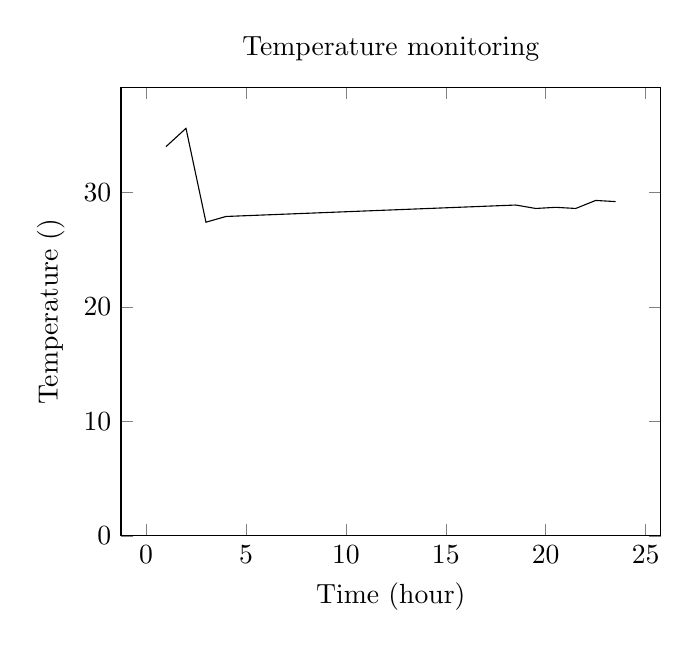
\begin{tikzpicture}[]
        \begin{axis}[title={Temperature monitoring}, ylabel=Temperature (\si{\celsius}) , xlabel=Time (hour), legend pos = south east, ymin=0]
            \addplot[] table{
            1	34.0
            2	35.6
            3	27.4
            4	27.9
            18.5	28.9
            19.5	28.6
            20.5	28.7
            21.5	28.6
            22.5	29.3
            23.5	29.2
            };
        \end{axis}
    \end{tikzpicture}
\end{figure}

The prototype was set up as described in section 4.3, and temperature of the bioreactor was taken at regular interval. A graph of the recorded temperature was plotted. As it can be observed from the graph, the temperature raised quickly at the beginning, reaching 35.6\si{\celsius} two hours after starting. This temperature was unexpected, and we decided to turn the heating plate down to 30 \si{\celsius} instead. Straight after that temperature dropped down to 27.4\si{\celsius}, and after five hours started it became steady, maintain in the range of 28.5-29.5 \si{\celsius}, which is out desired temperature range. 

\subsubsection{Fouling prevention techniques}
Fouling is the accumulation of unwanted materials such as scale, biomass and insoluble salts, on the internal or external surfaces of reactors. Fouling significantly impacts the efficiency of the reactors and increases the thermal resistance reducing the flow of heat. One technique to prevent fouling from occurring would be to use anti-fouling coatings such as Notak\texttrademark\ and Dursan\textsuperscript \textregistered\  which can be applied to the metal, ceramic and glass surface of the reactor. The anti-fouling coating is initially introduced as a gas then penetrates on the surface of the reactor to create a micro thin coating which bonds to the surface. This then reduces the risk of fouling from occurring as the coating can act as a barrier. Another method to prevent fouling from occurring is through the material selection when designing the equipment. Using materials that do not easily corrode or using materials with a low-fouling surface such as surfaces with ions, very smooth surfaces or surfaces of low surface energy will reduce the chance of fouling from occurring \cite{Ibrahim12}. If fouling has already occurred steam cleaning would assist in reducing the unwanted materials on the surfaces of the equipment, however this is not always effective and impacts the process productivity \cite{KillcrossMartin2012CPT}.